% Options for packages loaded elsewhere
\PassOptionsToPackage{unicode}{hyperref}
\PassOptionsToPackage{hyphens}{url}
\PassOptionsToPackage{dvipsnames,svgnames,x11names}{xcolor}
%
\documentclass[
  ignorenonframetext,
]{beamer}
\usepackage{pgfpages}
\setbeamertemplate{caption}[numbered]
\setbeamertemplate{caption label separator}{: }
\setbeamercolor{caption name}{fg=normal text.fg}
\beamertemplatenavigationsymbolsempty
% Prevent slide breaks in the middle of a paragraph
\widowpenalties 1 10000
\raggedbottom
\setbeamertemplate{part page}{
  \centering
  \begin{beamercolorbox}[sep=16pt,center]{part title}
    \usebeamerfont{part title}\insertpart\par
  \end{beamercolorbox}
}
\setbeamertemplate{section page}{
  \centering
  \begin{beamercolorbox}[sep=12pt,center]{part title}
    \usebeamerfont{section title}\insertsection\par
  \end{beamercolorbox}
}
\setbeamertemplate{subsection page}{
  \centering
  \begin{beamercolorbox}[sep=8pt,center]{part title}
    \usebeamerfont{subsection title}\insertsubsection\par
  \end{beamercolorbox}
}
\AtBeginPart{
  \frame{\partpage}
}
\AtBeginSection{
  \ifbibliography
  \else
    \frame{\sectionpage}
  \fi
}
\AtBeginSubsection{
  \frame{\subsectionpage}
}
\usepackage{amsmath,amssymb}
\usepackage{lmodern}
\usepackage{iftex}
\ifPDFTeX
  \usepackage[T1]{fontenc}
  \usepackage[utf8]{inputenc}
  \usepackage{textcomp} % provide euro and other symbols
\else % if luatex or xetex
  \usepackage{unicode-math}
  \defaultfontfeatures{Scale=MatchLowercase}
  \defaultfontfeatures[\rmfamily]{Ligatures=TeX,Scale=1}
\fi
% Use upquote if available, for straight quotes in verbatim environments
\IfFileExists{upquote.sty}{\usepackage{upquote}}{}
\IfFileExists{microtype.sty}{% use microtype if available
  \usepackage[]{microtype}
  \UseMicrotypeSet[protrusion]{basicmath} % disable protrusion for tt fonts
}{}
\makeatletter
\@ifundefined{KOMAClassName}{% if non-KOMA class
  \IfFileExists{parskip.sty}{%
    \usepackage{parskip}
  }{% else
    \setlength{\parindent}{0pt}
    \setlength{\parskip}{6pt plus 2pt minus 1pt}}
}{% if KOMA class
  \KOMAoptions{parskip=half}}
\makeatother
\usepackage{xcolor}
\newif\ifbibliography
\usepackage{color}
\usepackage{fancyvrb}
\newcommand{\VerbBar}{|}
\newcommand{\VERB}{\Verb[commandchars=\\\{\}]}
\DefineVerbatimEnvironment{Highlighting}{Verbatim}{commandchars=\\\{\}}
% Add ',fontsize=\small' for more characters per line
\usepackage{framed}
\definecolor{shadecolor}{RGB}{248,248,248}
\newenvironment{Shaded}{\begin{snugshade}}{\end{snugshade}}
\newcommand{\AlertTok}[1]{\textcolor[rgb]{0.94,0.16,0.16}{#1}}
\newcommand{\AnnotationTok}[1]{\textcolor[rgb]{0.56,0.35,0.01}{\textbf{\textit{#1}}}}
\newcommand{\AttributeTok}[1]{\textcolor[rgb]{0.77,0.63,0.00}{#1}}
\newcommand{\BaseNTok}[1]{\textcolor[rgb]{0.00,0.00,0.81}{#1}}
\newcommand{\BuiltInTok}[1]{#1}
\newcommand{\CharTok}[1]{\textcolor[rgb]{0.31,0.60,0.02}{#1}}
\newcommand{\CommentTok}[1]{\textcolor[rgb]{0.56,0.35,0.01}{\textit{#1}}}
\newcommand{\CommentVarTok}[1]{\textcolor[rgb]{0.56,0.35,0.01}{\textbf{\textit{#1}}}}
\newcommand{\ConstantTok}[1]{\textcolor[rgb]{0.00,0.00,0.00}{#1}}
\newcommand{\ControlFlowTok}[1]{\textcolor[rgb]{0.13,0.29,0.53}{\textbf{#1}}}
\newcommand{\DataTypeTok}[1]{\textcolor[rgb]{0.13,0.29,0.53}{#1}}
\newcommand{\DecValTok}[1]{\textcolor[rgb]{0.00,0.00,0.81}{#1}}
\newcommand{\DocumentationTok}[1]{\textcolor[rgb]{0.56,0.35,0.01}{\textbf{\textit{#1}}}}
\newcommand{\ErrorTok}[1]{\textcolor[rgb]{0.64,0.00,0.00}{\textbf{#1}}}
\newcommand{\ExtensionTok}[1]{#1}
\newcommand{\FloatTok}[1]{\textcolor[rgb]{0.00,0.00,0.81}{#1}}
\newcommand{\FunctionTok}[1]{\textcolor[rgb]{0.00,0.00,0.00}{#1}}
\newcommand{\ImportTok}[1]{#1}
\newcommand{\InformationTok}[1]{\textcolor[rgb]{0.56,0.35,0.01}{\textbf{\textit{#1}}}}
\newcommand{\KeywordTok}[1]{\textcolor[rgb]{0.13,0.29,0.53}{\textbf{#1}}}
\newcommand{\NormalTok}[1]{#1}
\newcommand{\OperatorTok}[1]{\textcolor[rgb]{0.81,0.36,0.00}{\textbf{#1}}}
\newcommand{\OtherTok}[1]{\textcolor[rgb]{0.56,0.35,0.01}{#1}}
\newcommand{\PreprocessorTok}[1]{\textcolor[rgb]{0.56,0.35,0.01}{\textit{#1}}}
\newcommand{\RegionMarkerTok}[1]{#1}
\newcommand{\SpecialCharTok}[1]{\textcolor[rgb]{0.00,0.00,0.00}{#1}}
\newcommand{\SpecialStringTok}[1]{\textcolor[rgb]{0.31,0.60,0.02}{#1}}
\newcommand{\StringTok}[1]{\textcolor[rgb]{0.31,0.60,0.02}{#1}}
\newcommand{\VariableTok}[1]{\textcolor[rgb]{0.00,0.00,0.00}{#1}}
\newcommand{\VerbatimStringTok}[1]{\textcolor[rgb]{0.31,0.60,0.02}{#1}}
\newcommand{\WarningTok}[1]{\textcolor[rgb]{0.56,0.35,0.01}{\textbf{\textit{#1}}}}
\usepackage{graphicx}
\makeatletter
\def\maxwidth{\ifdim\Gin@nat@width>\linewidth\linewidth\else\Gin@nat@width\fi}
\def\maxheight{\ifdim\Gin@nat@height>\textheight\textheight\else\Gin@nat@height\fi}
\makeatother
% Scale images if necessary, so that they will not overflow the page
% margins by default, and it is still possible to overwrite the defaults
% using explicit options in \includegraphics[width, height, ...]{}
\setkeys{Gin}{width=\maxwidth,height=\maxheight,keepaspectratio}
% Set default figure placement to htbp
\makeatletter
\def\fps@figure{htbp}
\makeatother
\setlength{\emergencystretch}{3em} % prevent overfull lines
\providecommand{\tightlist}{%
  \setlength{\itemsep}{0pt}\setlength{\parskip}{0pt}}
\setcounter{secnumdepth}{-\maxdimen} % remove section numbering
\usepackage{graphicx}
\usepackage{bm}
\usepackage{array}
\usepackage{amsmath}
\usepackage{amsthm}
\usepackage{amsfonts}
\usepackage{amssymb}
\usepackage{tikz-cd}
\usepackage{url}
\definecolor{foreground}{RGB}{255,255,255}
\definecolor{background}{RGB}{34,28,54}
\definecolor{title}{RGB}{105,165,255}
\definecolor{gray}{RGB}{175,175,175}
\definecolor{lightgray}{RGB}{225,225,225}
\definecolor{subtitle}{RGB}{232,234,255}
\definecolor{hilight}{RGB}{112,224,255}
\definecolor{vhilight}{RGB}{255,111,207}
\setbeamertemplate{footline}[page number]
\ifLuaTeX
  \usepackage{selnolig}  % disable illegal ligatures
\fi
\IfFileExists{bookmark.sty}{\usepackage{bookmark}}{\usepackage{hyperref}}
\IfFileExists{xurl.sty}{\usepackage{xurl}}{} % add URL line breaks if available
\urlstyle{same} % disable monospaced font for URLs
\hypersetup{
  pdftitle={STAT 528 - Advanced Regression Analysis II},
  pdfauthor={Multinomial response regression (part I)},
  colorlinks=true,
  linkcolor={Maroon},
  filecolor={Maroon},
  citecolor={Blue},
  urlcolor={blue},
  pdfcreator={LaTeX via pandoc}}

\title{STAT 528 - Advanced Regression Analysis II}
\author{Multinomial response regression (part I)}
\date{}
\institute{Daniel J. Eck\\
Department of Statistics\\
University of Illinois}

\begin{document}
\frame{\titlepage}

\begin{frame}
\newcommand{\R}{\mathbb{R}}
\newcommand{\Prob}{\mathbb{P}}
\newcommand{\Proj}{\textbf{P}}
\newcommand{\Hcal}{\mathcal{H}}
\newcommand{\rootn}{\sqrt{n}}
\newcommand{\p}{\mathbf{p}}
\newcommand{\E}{\text{E}}
\newcommand{\Var}{\text{Var}}
\newcommand{\Cov}{\text{Cov}}
\newcommand{\mubf}{\bm{\mu}}
\newcommand{\logit}{\text{logit}}

\newtheorem{cor}{Corollary}
\newtheorem{lem}{Lemma}
\newtheorem{thm}{Theorem}
\newtheorem{defn}{Definition}
\newtheorem{prop}{Proposition}
\end{frame}

\begin{frame}{Last time}
\protect\hypertarget{last-time}{}
\begin{itemize}
\tightlist
\item
  nominal responses
\item
  Multinomial regression via baseline-category logistic model
\item
  data analysis
\end{itemize}
\end{frame}

\begin{frame}{Learning Objectives Today}
\protect\hypertarget{learning-objectives-today}{}
\begin{itemize}
\tightlist
\item
  ordinal responses
\item
  proportional-odds model
\item
  data analysis
\end{itemize}

\vspace{12pt}

This slide deck will only contain data analysis. The lecture will be
largely on the blackboard.
\end{frame}

\begin{frame}{R Example: Happiness and Traumatic Events}
\protect\hypertarget{r-example-happiness-and-traumatic-events}{}
The response variable happiness is an ordinal categorical variable
indicating the current happiness level of the individual:

\begin{itemize}
\tightlist
\item
  1 if very happy
\item
  2 if pretty happy
\item
  3 if not too happy
\end{itemize}

\vspace{12pt}

Here trauma is a count of the number of traumatic events that the
individual faced in the previous year.

\vspace{12pt}

The control variable is a binary categorical variable (race) that was
deemed important by the researchers who conducted the study (given two
levels: 0 if in A; 1 if in B).
\end{frame}

\begin{frame}[fragile]{}
\protect\hypertarget{section}{}
We load in the data

\vspace{12pt}
\tiny

\begin{Shaded}
\begin{Highlighting}[]
\NormalTok{happiness }\OtherTok{\textless{}{-}} \FunctionTok{read.table}\NormalTok{(}\StringTok{"happiness.txt"}\NormalTok{, }\AttributeTok{header=}\ConstantTok{TRUE}\NormalTok{)}
\end{Highlighting}
\end{Shaded}

\vspace{12pt}
\normalsize

and display the first 10 rows:

\vspace{12pt}
\tiny

\begin{Shaded}
\begin{Highlighting}[]
\FunctionTok{head}\NormalTok{(happiness, }\DecValTok{10}\NormalTok{)}
\end{Highlighting}
\end{Shaded}

\begin{verbatim}
##    control trauma happy
## 1        0      0     1
## 2        0      0     1
## 3        0      0     1
## 4        0      0     1
## 5        0      0     1
## 6        0      0     1
## 7        0      0     1
## 8        0      0     2
## 9        0      0     2
## 10       0      0     2
\end{verbatim}
\end{frame}

\begin{frame}[fragile]{}
\protect\hypertarget{section-1}{}
We load in \texttt{VGAM} and fit the proportional-odds model

\vspace{12pt}
\tiny

\begin{Shaded}
\begin{Highlighting}[]
\FunctionTok{library}\NormalTok{(VGAM)}
\NormalTok{mod }\OtherTok{\textless{}{-}} \FunctionTok{vglm}\NormalTok{(happy }\SpecialCharTok{\textasciitilde{}}\NormalTok{ trauma }\SpecialCharTok{+}\NormalTok{ control, }\AttributeTok{family=}\FunctionTok{propodds}\NormalTok{(}\AttributeTok{reverse=}\ConstantTok{FALSE}\NormalTok{),}
            \AttributeTok{data=}\NormalTok{happiness)}
\FunctionTok{summary}\NormalTok{(mod)}
\end{Highlighting}
\end{Shaded}

\begin{verbatim}
## 
## Call:
## vglm(formula = happy ~ trauma + control, family = propodds(reverse = FALSE), 
##     data = happiness)
## 
## Coefficients: 
##               Estimate Std. Error z value Pr(>|z|)    
## (Intercept):1  -0.5181     0.3382  -1.532  0.12552    
## (Intercept):2   3.4006     0.5648   6.021 1.74e-09 ***
## trauma         -0.4056     0.1809  -2.242  0.02493 *  
## control        -2.0361     0.6911  -2.946  0.00322 ** 
## ---
## Signif. codes:  0 '***' 0.001 '**' 0.01 '*' 0.05 '.' 0.1 ' ' 1
## 
## Names of linear predictors: logitlink(P[Y<=1]), logitlink(P[Y<=2])
## 
## Residual deviance: 148.407 on 190 degrees of freedom
## 
## Log-likelihood: -74.2035 on 190 degrees of freedom
## 
## Number of Fisher scoring iterations: 5 
## 
## No Hauck-Donner effect found in any of the estimates
## 
## 
## Exponentiated coefficients:
##    trauma   control 
## 0.6665934 0.1305338
\end{verbatim}
\end{frame}

\begin{frame}[fragile]{}
\protect\hypertarget{section-2}{}
A LRT suggests that our model fits the data better than a saturated
model.

\vspace{12pt}
\small

\begin{Shaded}
\begin{Highlighting}[]
\FunctionTok{pchisq}\NormalTok{(}\FunctionTok{deviance}\NormalTok{(mod), }\FunctionTok{df.residual}\NormalTok{(mod), }\AttributeTok{lower =} \ConstantTok{FALSE}\NormalTok{)}
\end{Highlighting}
\end{Shaded}

\begin{verbatim}
## [1] 0.9886371
\end{verbatim}
\end{frame}

\begin{frame}{}
\protect\hypertarget{section-3}{}
In our notation, the estimates are

\begin{align*}
\begin{array}{c}
  \hat\alpha_1 \approx -0.518 \\
  \hat\alpha_2 \approx 3.401
\end{array} \qquad \hat\beta \approx \left(\begin{array}{c}
  -0.406 \\
  -2.036
\end{array}\right)
\end{align*}

\vspace{12pt}

where \[
  x = \left(\begin{array}{c}
  \text{trauma} \\
  \text{control}
\end{array}\right).
\]
\end{frame}

\begin{frame}[fragile]{}
\protect\hypertarget{section-4}{}
Thus happiness is estimated lower (\(Y\) is estimated to be larger) as
trauma increases.

\vspace{12pt}

We can estimate the odds of ``very happy'\,' for control category A
(coded 0) relative to control category B (coded 1) with trauma held
fixed, and a Wald 95\% confidence interval for these estimates:

\vspace{12pt}
\tiny

\begin{Shaded}
\begin{Highlighting}[]
\FunctionTok{exp}\NormalTok{(}\FloatTok{2.036}\NormalTok{)}
\end{Highlighting}
\end{Shaded}

\begin{verbatim}
## [1] 7.659908
\end{verbatim}

\begin{Shaded}
\begin{Highlighting}[]
\FunctionTok{exp}\NormalTok{(}\FloatTok{2.036} \SpecialCharTok{+} \FunctionTok{c}\NormalTok{(}\SpecialCharTok{{-}}\DecValTok{1}\NormalTok{,}\DecValTok{1}\NormalTok{) }\SpecialCharTok{*} \FunctionTok{qnorm}\NormalTok{(}\FloatTok{0.975}\NormalTok{) }\SpecialCharTok{*} \FloatTok{0.691}\NormalTok{)}
\end{Highlighting}
\end{Shaded}

\begin{verbatim}
## [1]  1.977167 29.675895
\end{verbatim}

\vspace{12pt}
\normalsize

The control variable (race) has a large effect on happiness
\end{frame}

\begin{frame}[fragile]{}
\protect\hypertarget{section-5}{}
We can do likelihood ratio tests as before

\vspace{12pt}
\tiny

\begin{Shaded}
\begin{Highlighting}[]
\NormalTok{modred }\OtherTok{\textless{}{-}} \FunctionTok{vglm}\NormalTok{(happy }\SpecialCharTok{\textasciitilde{}}\NormalTok{ trauma, }\AttributeTok{family=}\FunctionTok{propodds}\NormalTok{(}\AttributeTok{reverse=}\ConstantTok{FALSE}\NormalTok{),}
               \AttributeTok{data=}\NormalTok{happiness)}
\NormalTok{llrts }\OtherTok{\textless{}{-}} \FunctionTok{deviance}\NormalTok{(modred) }\SpecialCharTok{{-}} \FunctionTok{deviance}\NormalTok{(mod)}
\NormalTok{llrts.df }\OtherTok{\textless{}{-}} \FunctionTok{df.residual}\NormalTok{(modred) }\SpecialCharTok{{-}} \FunctionTok{df.residual}\NormalTok{(mod)}
\NormalTok{llrts}
\end{Highlighting}
\end{Shaded}

\begin{verbatim}
## [1] 9.231169
\end{verbatim}

\begin{Shaded}
\begin{Highlighting}[]
\NormalTok{llrts.df}
\end{Highlighting}
\end{Shaded}

\begin{verbatim}
## [1] 1
\end{verbatim}

\begin{Shaded}
\begin{Highlighting}[]
\DecValTok{1} \SpecialCharTok{{-}} \FunctionTok{pchisq}\NormalTok{(llrts, llrts.df)}
\end{Highlighting}
\end{Shaded}

\begin{verbatim}
## [1] 0.002379297
\end{verbatim}
\end{frame}

\begin{frame}[fragile]{}
\protect\hypertarget{section-6}{}
We can also graph probability curves (versus trauma) by happiness
category and control:

\vspace{12pt}
\tiny

\begin{Shaded}
\begin{Highlighting}[]
\FunctionTok{curve}\NormalTok{(}\FunctionTok{predict}\NormalTok{(mod, }\FunctionTok{data.frame}\NormalTok{(}\AttributeTok{trauma=}\NormalTok{x,}\AttributeTok{control=}\DecValTok{0}\NormalTok{), }\AttributeTok{type=}\StringTok{"response"}\NormalTok{)[,}\DecValTok{1}\NormalTok{],}
      \AttributeTok{xlab=}\StringTok{"Trauma"}\NormalTok{, }\AttributeTok{ylab=}\StringTok{"Probability"}\NormalTok{,}
      \AttributeTok{xlim=}\FunctionTok{range}\NormalTok{(happiness}\SpecialCharTok{$}\NormalTok{trauma), }\AttributeTok{ylim=}\FunctionTok{c}\NormalTok{(}\DecValTok{0}\NormalTok{,}\DecValTok{1}\NormalTok{))}
\FunctionTok{curve}\NormalTok{(}\FunctionTok{predict}\NormalTok{(mod, }\FunctionTok{data.frame}\NormalTok{(}\AttributeTok{trauma=}\NormalTok{x,}\AttributeTok{control=}\DecValTok{0}\NormalTok{), }\AttributeTok{type=}\StringTok{"response"}\NormalTok{)[,}\DecValTok{2}\NormalTok{],}
      \AttributeTok{add=}\ConstantTok{TRUE}\NormalTok{, }\AttributeTok{col=}\StringTok{"red"}\NormalTok{)}
\FunctionTok{curve}\NormalTok{(}\FunctionTok{predict}\NormalTok{(mod, }\FunctionTok{data.frame}\NormalTok{(}\AttributeTok{trauma=}\NormalTok{x,}\AttributeTok{control=}\DecValTok{0}\NormalTok{), }\AttributeTok{type=}\StringTok{"response"}\NormalTok{)[,}\DecValTok{3}\NormalTok{],}
      \AttributeTok{add=}\ConstantTok{TRUE}\NormalTok{, }\AttributeTok{col=}\StringTok{"blue"}\NormalTok{)}
\FunctionTok{curve}\NormalTok{(}\FunctionTok{predict}\NormalTok{(mod, }\FunctionTok{data.frame}\NormalTok{(}\AttributeTok{trauma=}\NormalTok{x,}\AttributeTok{control=}\DecValTok{1}\NormalTok{), }\AttributeTok{type=}\StringTok{"response"}\NormalTok{)[,}\DecValTok{1}\NormalTok{],}
      \AttributeTok{add=}\ConstantTok{TRUE}\NormalTok{, }\AttributeTok{lty=}\DecValTok{2}\NormalTok{)}
\FunctionTok{curve}\NormalTok{(}\FunctionTok{predict}\NormalTok{(mod, }\FunctionTok{data.frame}\NormalTok{(}\AttributeTok{trauma=}\NormalTok{x,}\AttributeTok{control=}\DecValTok{1}\NormalTok{), }\AttributeTok{type=}\StringTok{"response"}\NormalTok{)[,}\DecValTok{2}\NormalTok{],}
      \AttributeTok{add=}\ConstantTok{TRUE}\NormalTok{, }\AttributeTok{col=}\StringTok{"red"}\NormalTok{, }\AttributeTok{lty=}\DecValTok{2}\NormalTok{)}
\FunctionTok{curve}\NormalTok{(}\FunctionTok{predict}\NormalTok{(mod, }\FunctionTok{data.frame}\NormalTok{(}\AttributeTok{trauma=}\NormalTok{x,}\AttributeTok{control=}\DecValTok{1}\NormalTok{), }\AttributeTok{type=}\StringTok{"response"}\NormalTok{)[,}\DecValTok{3}\NormalTok{],}
      \AttributeTok{add=}\ConstantTok{TRUE}\NormalTok{, }\AttributeTok{col=}\StringTok{"blue"}\NormalTok{, }\AttributeTok{lty=}\DecValTok{2}\NormalTok{)}
\FunctionTok{legend}\NormalTok{(}\StringTok{"topright"}\NormalTok{, }\FunctionTok{c}\NormalTok{(}\StringTok{"A"}\NormalTok{,}\StringTok{"B"}\NormalTok{), }\AttributeTok{lty=}\DecValTok{1}\SpecialCharTok{:}\DecValTok{2}\NormalTok{)}
\FunctionTok{legend}\NormalTok{(}\StringTok{"topleft"}\NormalTok{, }\FunctionTok{c}\NormalTok{(}\StringTok{"Very Happy"}\NormalTok{,}\StringTok{"Pretty Happy"}\NormalTok{,}\StringTok{"Not Too Happy"}\NormalTok{), }\AttributeTok{lty=}\DecValTok{1}\NormalTok{,}
       \AttributeTok{col=}\FunctionTok{c}\NormalTok{(}\StringTok{"black"}\NormalTok{,}\StringTok{"red"}\NormalTok{,}\StringTok{"blue"}\NormalTok{))}
\end{Highlighting}
\end{Shaded}
\end{frame}

\begin{frame}{}
\protect\hypertarget{section-7}{}
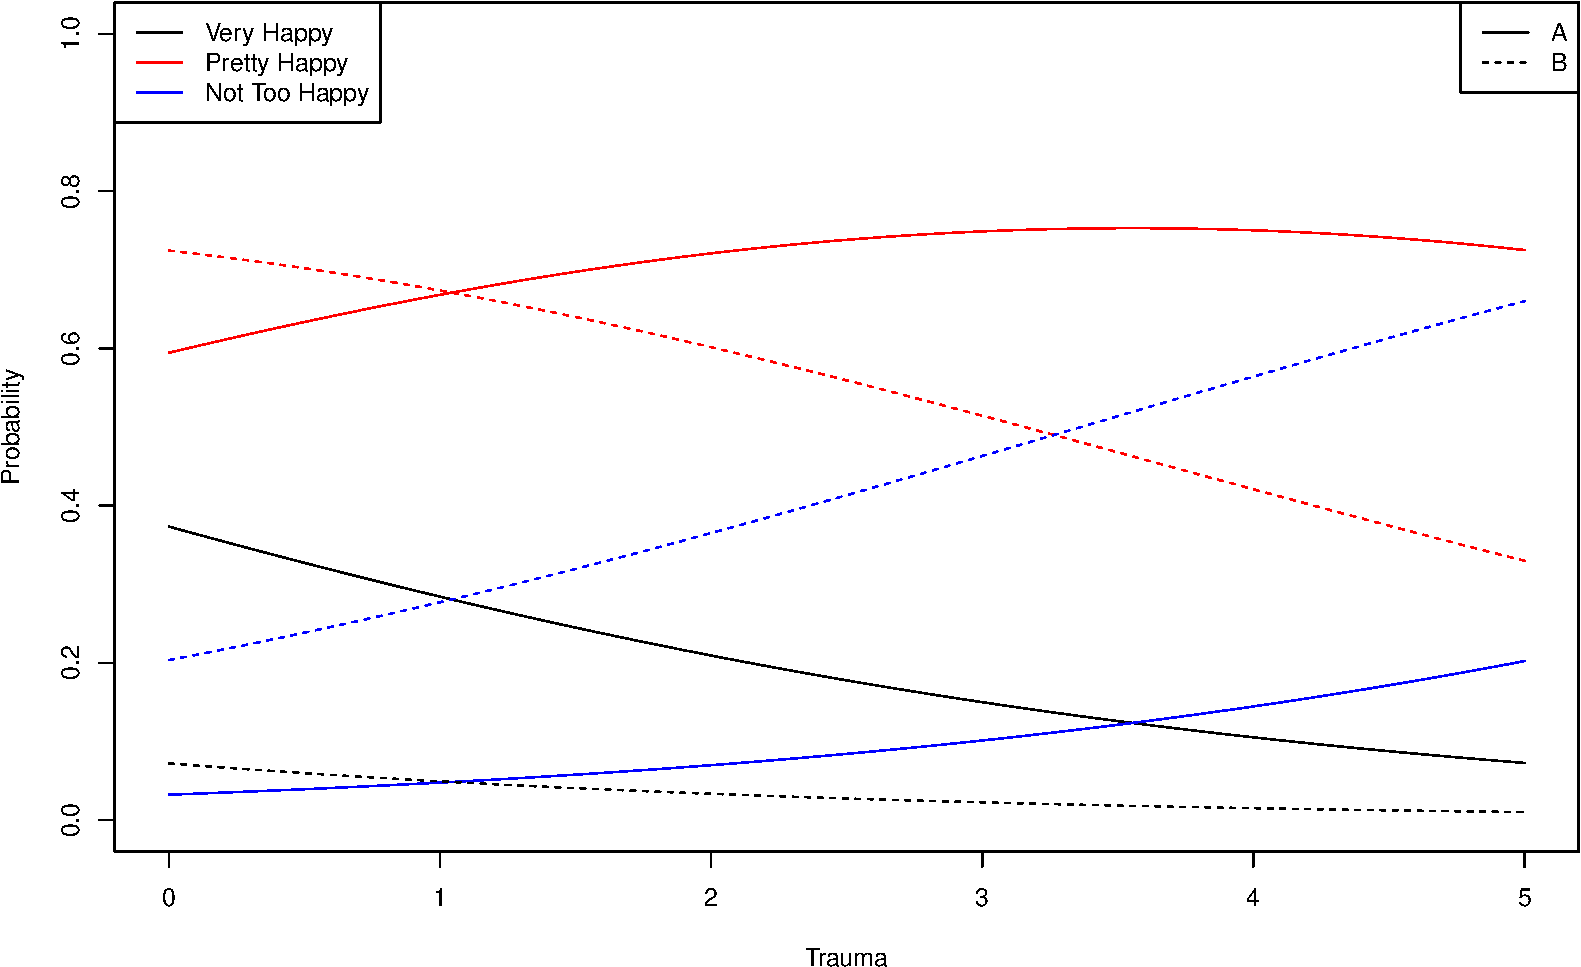
\includegraphics{week6_p2_files/figure-beamer/unnamed-chunk-9-1.pdf}
\end{frame}

\begin{frame}[fragile]{}
\protect\hypertarget{section-8}{}
We can check the assumption of proportional odds by comparison with a
model that does not assume it:

\vspace{12pt}
\tiny

\begin{Shaded}
\begin{Highlighting}[]
\NormalTok{modnotprop }\OtherTok{\textless{}{-}} \FunctionTok{vglm}\NormalTok{(happy }\SpecialCharTok{\textasciitilde{}}\NormalTok{ trauma }\SpecialCharTok{+}\NormalTok{ control, }\AttributeTok{family=}\FunctionTok{cumulative}\NormalTok{(}\AttributeTok{parallel=}\ConstantTok{FALSE}\NormalTok{),}
                   \AttributeTok{data=}\NormalTok{happiness)}
\FunctionTok{summary}\NormalTok{(modnotprop)}
\end{Highlighting}
\end{Shaded}

\begin{verbatim}
## 
## Call:
## vglm(formula = happy ~ trauma + control, family = cumulative(parallel = FALSE), 
##     data = happiness)
## 
## Coefficients: 
##                Estimate Std. Error z value Pr(>|z|)    
## (Intercept):1   -0.5661     0.3662  -1.546   0.1221    
## (Intercept):2    3.4837     0.7595   4.587  4.5e-06 ***
## trauma:1        -0.3409     0.2124  -1.605   0.1086    
## trauma:2        -0.4836     0.2752  -1.757   0.0789 .  
## control:1      -16.8922  1358.1457      NA       NA    
## control:2       -1.8467     0.7628  -2.421   0.0155 *  
## ---
## Signif. codes:  0 '***' 0.001 '**' 0.01 '*' 0.05 '.' 0.1 ' ' 1
## 
## Names of linear predictors: logitlink(P[Y<=1]), logitlink(P[Y<=2])
## 
## Residual deviance: 146.9951 on 188 degrees of freedom
## 
## Log-likelihood: -73.4976 on 188 degrees of freedom
## 
## Number of Fisher scoring iterations: 17 
## 
## Warning: Hauck-Donner effect detected in the following estimate(s):
## '(Intercept):2', 'control:1'
## 
## 
## Exponentiated coefficients:
##     trauma:1     trauma:2    control:1    control:2 
## 7.111256e-01 6.165865e-01 4.611204e-08 1.577527e-01
\end{verbatim}
\end{frame}

\begin{frame}[fragile]{}
\protect\hypertarget{section-9}{}
Now perform the LRT. Keep in mind that forcing proportionality is more
restrictive than not enforcing it.

\vspace{12pt}
\tiny

\begin{Shaded}
\begin{Highlighting}[]
\NormalTok{llrts }\OtherTok{\textless{}{-}} \FunctionTok{deviance}\NormalTok{(mod) }\SpecialCharTok{{-}} \FunctionTok{deviance}\NormalTok{(modnotprop)}
\NormalTok{llrts.df }\OtherTok{\textless{}{-}} \FunctionTok{df.residual}\NormalTok{(mod) }\SpecialCharTok{{-}} \FunctionTok{df.residual}\NormalTok{(modnotprop)}
\NormalTok{llrts}
\end{Highlighting}
\end{Shaded}

\begin{verbatim}
## [1] 1.411892
\end{verbatim}

\begin{Shaded}
\begin{Highlighting}[]
\NormalTok{llrts.df}
\end{Highlighting}
\end{Shaded}

\begin{verbatim}
## [1] 2
\end{verbatim}

\begin{Shaded}
\begin{Highlighting}[]
\DecValTok{1} \SpecialCharTok{{-}} \FunctionTok{pchisq}\NormalTok{(llrts, llrts.df)}
\end{Highlighting}
\end{Shaded}

\begin{verbatim}
## [1] 0.4936413
\end{verbatim}

\vspace{12pt}
\normalsize

The proportional-odds model fits this data better.
\end{frame}

\begin{frame}[fragile]{}
\protect\hypertarget{section-10}{}
We can also fit a probit analog to the proportional-odds model

\vspace{12pt}
\tiny

\begin{Shaded}
\begin{Highlighting}[]
\NormalTok{mod.probit }\OtherTok{\textless{}{-}} \FunctionTok{vglm}\NormalTok{(happy }\SpecialCharTok{\textasciitilde{}}\NormalTok{ trauma }\SpecialCharTok{+}\NormalTok{ control,}
                   \AttributeTok{family=}\FunctionTok{cumulative}\NormalTok{(}\AttributeTok{link=}\StringTok{"probitlink"}\NormalTok{,}\AttributeTok{parallel=}\ConstantTok{TRUE}\NormalTok{),}
                   \AttributeTok{data=}\NormalTok{happiness)}
\FunctionTok{summary}\NormalTok{(mod.probit)}
\end{Highlighting}
\end{Shaded}

\begin{verbatim}
## 
## Call:
## vglm(formula = happy ~ trauma + control, family = cumulative(link = "probitlink", 
##     parallel = TRUE), data = happiness)
## 
## Coefficients: 
##               Estimate Std. Error z value Pr(>|z|)    
## (Intercept):1 -0.34808    0.20015  -1.739  0.08201 .  
## (Intercept):2  1.91607    0.28287   6.774 1.26e-11 ***
## trauma        -0.22131    0.09897  -2.236  0.02535 *  
## control       -1.15712    0.37872  -3.055  0.00225 ** 
## ---
## Signif. codes:  0 '***' 0.001 '**' 0.01 '*' 0.05 '.' 0.1 ' ' 1
## 
## Names of linear predictors: probitlink(P[Y<=1]), probitlink(P[Y<=2])
## 
## Residual deviance: 148.1066 on 190 degrees of freedom
## 
## Log-likelihood: -74.0533 on 190 degrees of freedom
## 
## Number of Fisher scoring iterations: 5 
## 
## No Hauck-Donner effect found in any of the estimates
## 
## 
## Exponentiated coefficients:
##    trauma   control 
## 0.8014668 0.3143908
\end{verbatim}
\end{frame}

\begin{frame}{}
\protect\hypertarget{section-11}{}
See notes \texttt{polr} implementation.
\end{frame}

\end{document}
